%
% state machine design
%

\documentclass[11pt]{article} 
\usepackage[dvips]{graphicx}
\usepackage{times}

\graphicspath{{./}{figs/}} 

\pagestyle{plain}

\addtolength{\hoffset}{-2cm}
\addtolength{\textwidth}{4cm}

\addtolength{\voffset}{-1.5cm}
\addtolength{\textheight}{3cm}

\setlength{\parindent}{0pt}
\setlength{\parskip}{11pt}

\title{PVFS2 State Machine Design Notes}
\author{PVFS Development Team}
\date{July 2002}

\begin{document}

\maketitle

\section{Introduction}

This document is to serve as a reference for the State Machine used in the PVFS2 server daemon.  The state
machine is used to process all (expected and unexpected) requests.  It will have the capabilities of
loading dynamic request processors as well as matching operations on opcode's or strings.

\section{Terminology}

In order for this document to make sense, a few terms must be defined.

\begin{description}
\item [Operation]: This is the overall task to be performed by the server.  It begins as an unexpected
message and the message contains the structure PVFS\_server\_req\_s.

\item [State]: From an operation standpoint a state consists of creating a new job with parameters contained within the buffer.  States should terminate with posting a job.  End states should clean up server\_op structures as well as any buffers.

\item [Job]: This refers to the usage of the job interface, a call to the job interface returns both a job\_return\_value (job\_status\_s) and a job\_post\_return\_value (int).  The job\_status\_s structure is passed throughout the functions as a pointer.  Once a structure is returned, the job interface will never modify it.  Therefore it is valid throughout the multiple calls through a state machine.  A function does not have to free the structure.

\item [Job Post Return Value (int)]: This is the value returned by the job post function at the end of each state.  It is used to determine the completion of an intermediate state and if the next state can be.  Values can be 0, 1, or -errno.  

\item [Job Return Value]: Value used in next\_state transition for determination of the next state.  There is no fixed set of values for this integer.  This value is found in ret-$\rangle$error\_code, where ret is of type job\_status\_s *. 

\item [Server State Array]: The array containing all individual Request State Arrays as well as associated
strings.  They are indexed by their op\_code, and can also be found by string references.

\item [Request State Array]:  All functions and return codes for a single Server Request.  Contained
within a PINT\_serv\_req\_s-$\rangle$state\_machine pointer.
\end{description}

\section{Design}

The state machine has two distinct types, one of which is a union used for the individual state machine
arrays as well as a structure which can manage multiple arrays at a higher level.

\subsection{Types}

\subsubsection{Server State Array}
The Server State Array is of type PINT\_serv\_req\_s which has the following members:

\begin{verbatim}
typedef struct PINT_serv_req_s
{
PINT_state_array_values *state_machine;
char *name;
void (*init_fun)(void);
} PINT_serv_req_s;
\end{verbatim}

\begin{description}
\item [PINT\_state\_array\_values *state\_machine]: The actual state machine array used by the
PINT\_state\_machine\_next() function.

\item [char *name]: The string reference to the operation.  Used for extended operations or when the
operation code is unknown or invalid.

\item [void init\_fun(void)]: A function pointer used to initialize corresponding state\_machine array. 
This function is called when PINT\_state\_machine\_init() is invoked.

\end{description}
 
\subsubsection{State Array Values}

The request state array consists of a union defined as the following.

\begin{verbatim}
typedef union PINT_state_array_values
   {
   int retVal;
   int (*handler)(PINT_server_op *s_op, job_status_s *r);
   union PINT_state_array_values *index;
   } PINT_state_array_values;
\end{verbatim}

\begin{description}

\item [retVal] The result of the last operation.  This is not to be confused with a function call to the job interface.  A call to the job interface determines the completion of that specific job.

\item [handler] The function to be called for the current state.

\item [index] The location of the next area of return values and corresponding functions.

\end{description}

\subsubsection{Server Op Structure}

Neither the job interface nor the state machine processor maintain the status of any job in between
requests.  Therefore, the server must maintain the in between state of each process.  This is done using a
structure called the server\_op and the details are below.

\begin{verbatim}
typedef struct PINT_server_op
   {
   int op;
   int strsize;
   bmi_addr_t addr;
   bmi_msg_tag_t tag;
   PINT_state_array_values location;
   struct PVFS_server_req_s *req;
   struct PVFS_server_resp_s *resp;
   struct unexpected_info *unexp_bmi_buff;
   } PINT_server_op;
\end{verbatim}

The fields in the structure are used as follows:

\begin{description}

\item[op] The op field is used to keep track of what request has been issued by the client.  Initially it
is used by the check\_dependencies part of the job interface to find the first state of the state machine.

\item[strsize] Used to maintain the size of all strings within a server response structure.

\item[addr] The bmi address of the client performing the request.

\item[tag] A BMI parameter required for all BMI messages sent from the server.

\item[location] A pointer in the specific state array for the operation.  Dereferencing this pointer holds
the value for the first possible return value of the previous job.  \emph{location+1} holds another
pointer to a location in the state array where the next function to be executed resides.

\item[req] The request structure provided by the client.  For more information see the Server Request
Protocol Document.

\item[resp] The response structure being worked on by the state machine.  For more information see the
Server Request Document.

\item[unexp\_bmi\_buff] The buffer that was posted initially to receive the unexpected message from a
client.  

\end{description}

\subsection{Functions}

The state machine interface has very few functions contained in it due to the associated pointer
arithmetic. They are as follows:

\begin{description}

\item [void PINT\_state\_machine\_init()]: This initializes the state machine linking in pointers to state
array structures that are statically compiled.

\item [void PINT\_state\_machine\_halt()]: This function frees all pointers within the large state array
structure including those dynamically created.

\item [int PINT\_state\_machine\_next(PINT\_server\_op *server\_op, job\_status\_r *r)]: Calls the next 
function associated with the return value of a job
call.  If there is the potential for an undefined state to be reached, this function expects a default
value to be stored in the array such that the next value in the array contains a pointer to handle the
undefined behavior.  The return value of this function is int and is passed back to the server daemon to
reflect the status of a job posted in the state that is executed.

\item [PINT\_state\_array\_values *PINT\_state\_machine\_locate(PINT\_server\_op *op)]: This returns the
state array indexed to the first return value so that PINT\_state\_machine\_next can operate once the
first function is called. \emph{If op not valid, should do string compare (if implemented). where is it in
server request proto?}

\item [int PINT\_state\_machine\_initialize\_unexpected(PINT\_server\_op *s\_op, job\_status\_s *ret)]:
Finalizes the setup for the server\_op, sets the location pointer for PINT\_state\_machine\_next and calls
the first function for the respective request.

\item [int PINT\_state\_machine\_load(char *filename� int major\_num)]:  This function can be used to
dynamically load a function into the state array.  If the major\_num is set to zero or if that position in
the state array is already allocated, then the function will return the new major number.  Otherwise the
function returns zero. /emph{not implemented}

\item [int PINT\_state\_machine\_getNext()]: Returns the first free major number in the state machine array. /emph{not implemented}

\end{description}

\subsection{Array Layout}

The array is arranged in a very organized manner.  We begin with the diagram shown in figure \ref{fig:array}.

\begin{figure}[ht]
\begin{center}
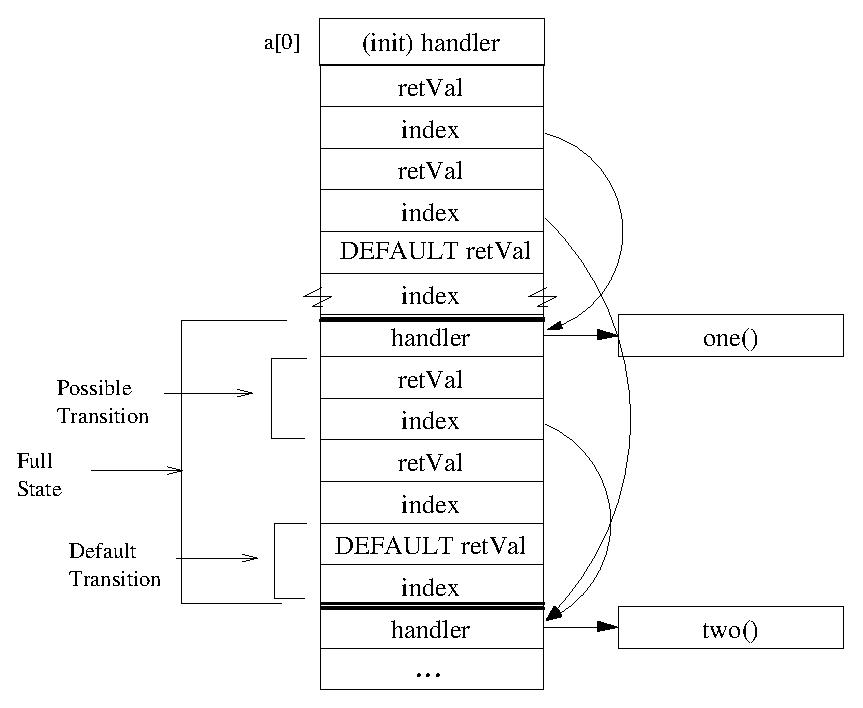
\includegraphics[scale=0.9]{arrayFig.eps}
\end{center}
\caption{Layout of a request state array \label{fig:array}}
\end{figure}

There are two very important concepts to notice.  The first entry of each request's state array 
\emph{must} be the initialization function for the state machine.  This function can expect a server\_op
structure where the BMI information and the PVFS\_server\_req\_s is set up.  \emph{semantics??}

\emph{where to malloc resp struct?  where to call check\_deps???}

\subsection{Macros}

To make the source code of the statically compiled array cleaner, macros were created.

\begin{description}
\item [set\_ptr(i,j,k)] Used to set a pointer in array i at index j to index k.  or i[j] = \&i[k]

\item [set\_fun(i,j,k)] Used to set a pointer in array i at index j to the function k.

\item [set\_ret(i,j,k)] Used to set a pointer in array i at index j to the integer k.

\item [STATE\_FXN\_HEAD(i)] Used to create a function with that name.  Can be used for both prototyping
and for coding.  Sets given parameters for the type contained within the union.

\item [STATE\_FXN\_RET(i)] Used to determine the ``return'' method.  At one point in time this was a jmp
command, but as of this document it simply returns the integer i.

\end{description}

\subsection{Operation of the State Machines}

The state machine itself has one function to control the transition of states in
the state machine.  This function operates with very little knowledge of the individual machines and
really compares predetermined output as well as undetermined (in the form of a default value) to force the
transitions.  PINT\_state\_machine\_next() assumes the location pointer within the server\_op struct
points to the first possible return value of the function that was previously called.  It begins by
comparing the return values:

\begin{verbatim}
PINT_state_array_values *loc = s->location.index;
while (loc->retVal != code_val && loc->retVal != DEFAULT_VALUE)
   loc += 2;
\end{verbatim}

Once we have found the next state to go to, we must update the server\_op structure, and call the next
function:

\begin{verbatim}
s->location.index = (loc + 1)->index + 1;
((s->location.index - 1)->handler)(s,r);
\end{verbatim}

Again, we know that loc currently has the return value or the default value matching our output.
Therefore the next state should be at loc+1.  Dereferencing that pointer and adding one gives us the first
possible return value of the function we are about to call.  Then, we call the next function.  Note this
is counter-intuitive in that the next function is called AFTER processing the previous functions return
values.

The PINT\_state\_machine\_next() function is called from inside the while loop from the main server
daemon.  This code appears in a loop, but a single execution of the loop looks like the following:

\begin{verbatim}
    s_op = my_user_ptrs[i];
    if(s_op->op == BMI_UNEXP)
    {

doWorkUnexp:
       ret = PINT_state_machine_initialize_unexpected(s_op,&status_jobs[i]);
       postBMIFlag = 1;

    }
    else
    {
       ret = PINT_state_machine_next(s_op,&status_jobs[i]);
    }
    while(ret == 1)
    {
       ret = PINT_state_machine_next(s_op,&status_jobs[i]);
    }

    if(ret < 0)
    {
       printf("Error on job %d, Return Code: %d\n",i,ret);
       goto doWorkUnexp;
    }
    if(postBMIFlag)
    {
       printf("Posting Another BMI Job\n");
       postBMIFlag = 0;
       ret = PINT_server_cp_bmi_unexp(s_op,&status_jobs[i]);
       if(ret == 1)
       {
          goto doWorkUnexp;
       }
    }


\end{verbatim}

\begin{figure}[h]
\begin{center}
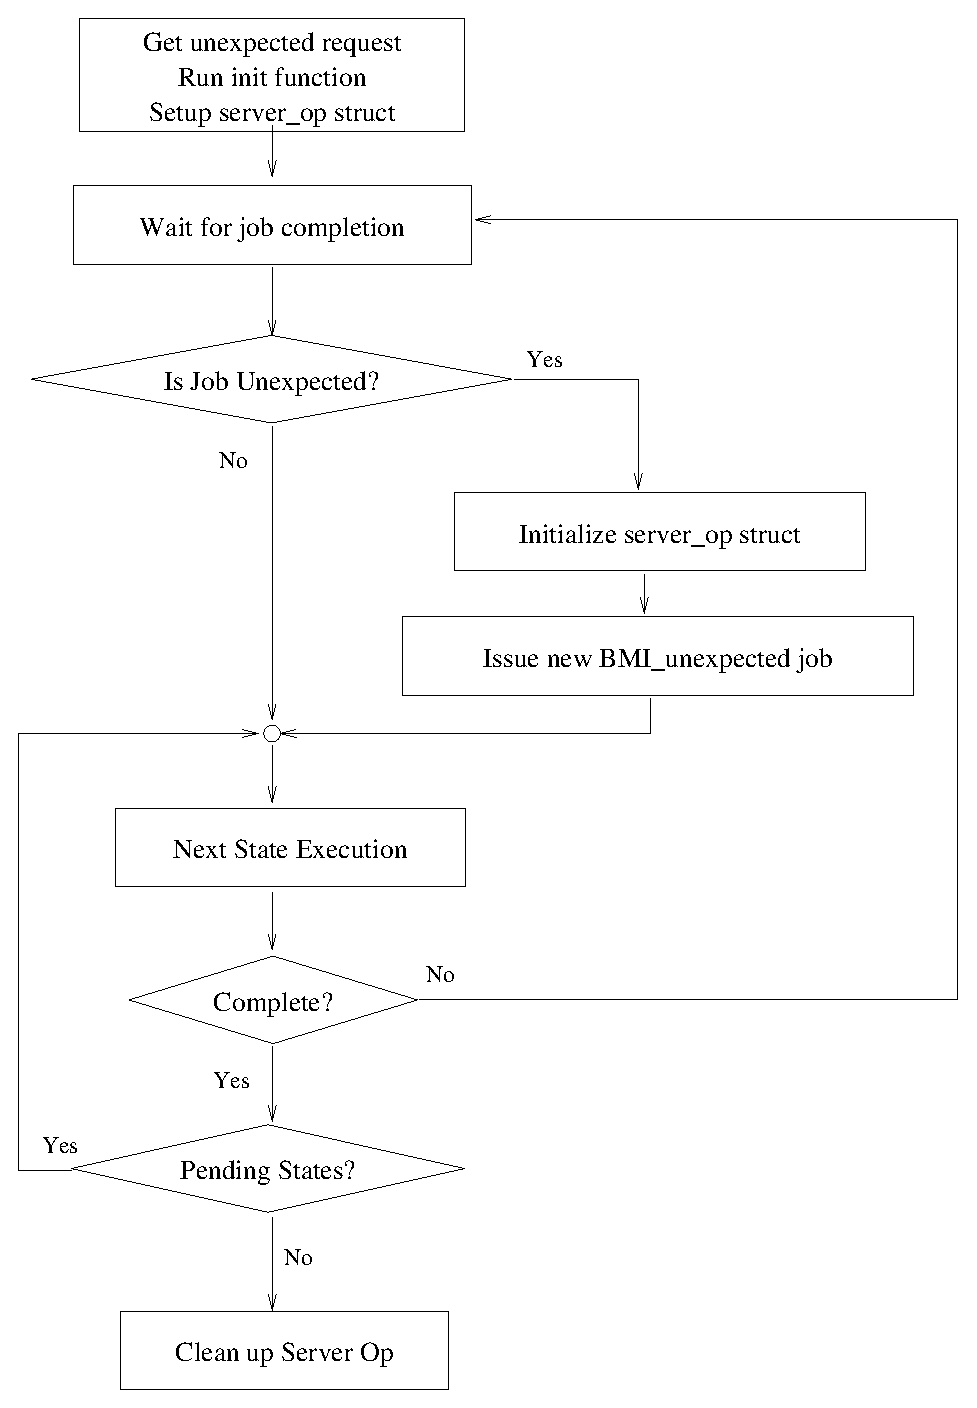
\includegraphics[scale=0.6]{stateExec2.eps}
\end{center}
\caption{How the State Machine works \label{fig:stateExec}}
\end{figure}

This code works by first looking at the server\_op.  If the structure has not been setup, we call
initialize on the structure to set it up to work properly with the state machine.  The initialize function
will call the first function required by that state machine.  Note also the postBMIFlag is set to one.
Now, if the structure has already been initialized, we simply call next on the structure.  Then, if that
state is complete (ret == 1), we continue processing that job.

Once the request state machine does not complete immediately, we check if we need to post a corresponding
unexpected request since the job we could have finished processing was unexpected.  Keeping in mind that
an unexpected job can post immediately, we check that condition and if true, initialize that request,
otherwise, go back to either a request that is completed, or wait for a request to complete.

The job interface currently does not have code provided for the check dependency.  This function is
expected to schedule requests as well as provide a level of coherence/ordering for operations
performed by clients.  Check dependencies will be discussed later as it is beyond the scope of this
document.

\section{Dynamic State Machines}

The state machine is designed to be portable, and will offer the ability to dynamically load new state
machines through two separate interfaces.  One way is obviously at run time to load these new modules
and/or on restart of the server.  The requirements of the module will be listed later in this section.
However, the other method of dynamic loading is through the server request protocol.  There has been
discussion of a privileged mode in which servers can communicate with each other without the clients
performing requests.  In this, I would propose that we allow servers to enhance their operations.  This
could also be done during the runtime of the server, but the semantics of that are
currently undefined.  Once the communication layers are defined, a more detailed
description of timing and semantics can be discussed. \emph{Check this out! Discussion time.}

The module must be laid out in such a way that the first value in the state array is the initialization
function for the specific request.  In other words, this function will be responsible for allocating
memory for the response structure and any other information it might need.  The module must also have in
it a function called \emph{init\_state\_machine} which when called with no parameters will return an array
for that state machine.  There is one other function that must be in place \emph{get\_state\_major\_num}
which returns the preferred major number of the request.  However, the state machine has the ultimate
decision of the major number if either the number returned is zero or the number is already taken by
another state machine.

\section{Auto-generation}

A state machine can be better designed when all transitions are mapped graphically.  In this scenario, dot
was used to perform just that task.  Dot is a directed graph specification language that can be used to
easily build these state machines graphically.  Because time is invested in building these graphs, another
tool was created to automatically build skeleton c-code for use once a graph was completed.

There are two ways of generating the skeleton code using the provided parser.  First, consider a very
trivial state machine where there are only two states.  The code for the graph is as follows:

\begin{verbatim}
digraph G {

   node0 [label = "start"];
	node1 [label = "end"];

	node0 -> node1;
	}
\end{verbatim}

When this graph is issued through dot, the following diagram shown in figure \ref{fig:state} results:

\begin{figure}[h]
\begin{center}
\includegraphics[scale=0.6]{simpleState.eps}
\end{center}
\caption{Simple State \label{fig:state}}
\end{figure}

Now, the parser could be run on this simple file, and the output would be as follows: 

\begin{verbatim}
/* This file has been generated by GPR */


/* 
 * (C) 2001 Clemson University and The University of Chicago 
 *
 * See COPYING in top-level directory.
 */


#include <state_machine.h>



STATE_FXN_HEAD(node0)
        {
        PINT_server_op *s_op = (PINT_server_op *) b;
        int job_ret_val;

        STATE_FXN_RET(job_ret_val);
        }

STATE_FXN_HEAD(node1)
        {
        PINT_server_op *s_op = (PINT_server_op *) b;
        int job_ret_val;

        STATE_FXN_RET(job_ret_val);
        }

\end{verbatim}

To make this code more usable, there are a few parameters we can add to the original graph.  The first
method is to change the actual names of the nodes such as:

\begin{verbatim}

digraph G {

   state_start [label = "start"];
	state_end [label = "end"];

	state_start -> state_end;
	}

\end{verbatim}

The other option is to set a variable within each node:

\begin{verbatim}

digraph G {

   node0 [label = "start" functName="state_start"];
	node1 [label = "end" functName="state_end"];

	node0 -> node1;
	}

\end{verbatim}

Either method will change the function names in the corresponding c-skeleton like so:

\begin{verbatim}

STATE_FXN_HEAD(state_start)

\end{verbatim}

One other parameter that
can be used is the code parameter.  If there is specific code that should be in the file, the code
parameter can be placed in the brackets and the code will be placed in the file in between the variable
declarations and the return() command.  

To build a state machine skeleton, the syntax is as follows:

\begin{verbatim}

~>gpr generateSkeleton.gpr "graph_name.graph" > "graph_skel.c"

\end{verbatim}

The GPR file is laid out quite simply, and upon inspection of the man page for gpr, all syntax will make sense.  

\section{Examples}
The following is an example of what should happen after the initialization 
of both a state machine and
then the configuration structure for a getconfig request.

Also shown is the getconfig array layout with all function mappings.

\begin{figure}[hb]
\begin{center}
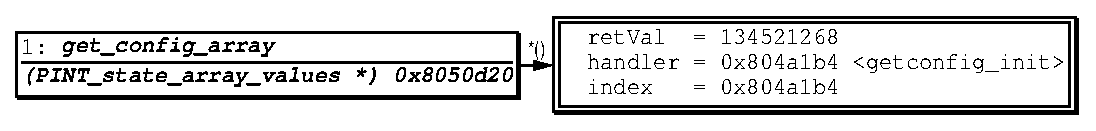
\includegraphics[scale=0.9]{getconfiginit.eps}
\end{center}
\caption{The Status of an array after init\_state\_machine \label{fig:stateInit}}
\end{figure}

\begin{figure}[h!]
\begin{center}
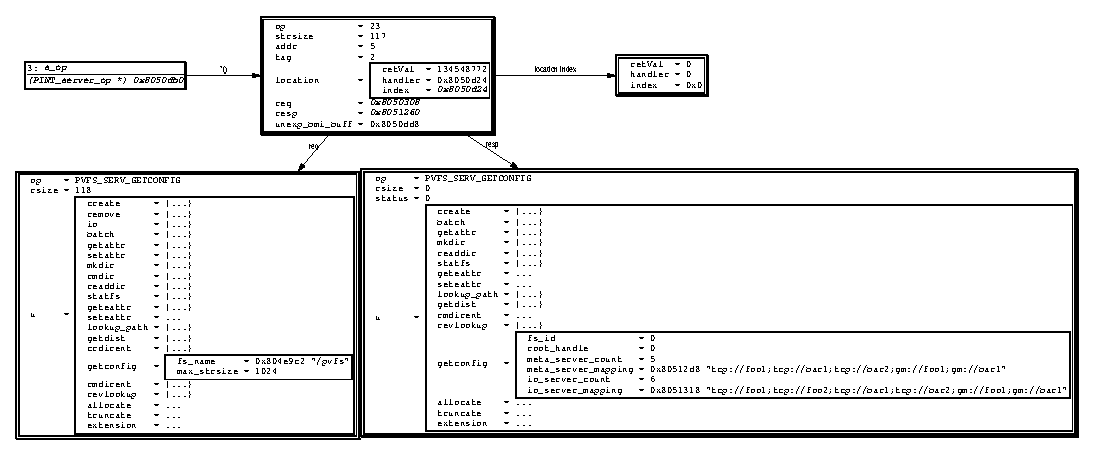
\includegraphics[scale=1.0]{getconfigservop.eps}
\end{center}
\caption{The Status of a server op after get\_config\_init \label{fig:getInit}}
\end{figure}

\begin{figure}[hb]
\begin{center}
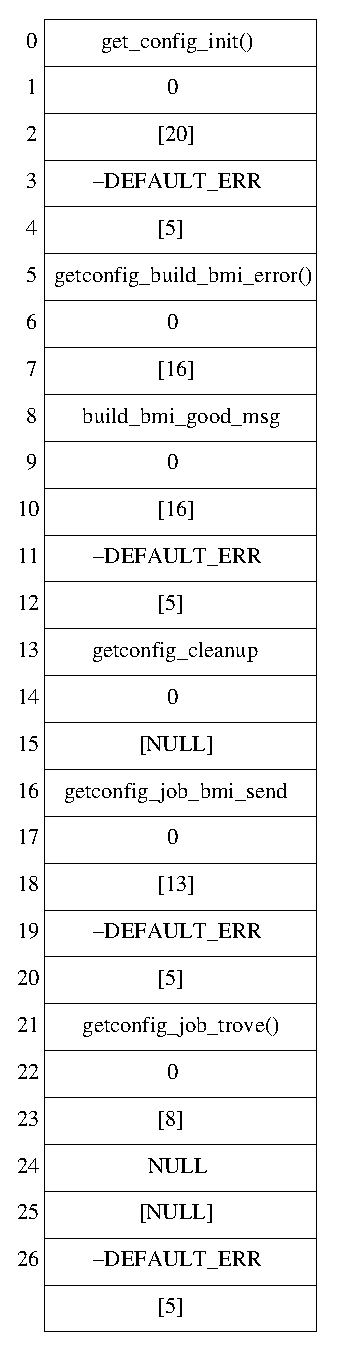
\includegraphics[scale=0.8]{get_configArrayLayout.eps}
\end{center}
\caption{Get\_config Array \label{fig:getArray}}
\end{figure}


%\section{Check Dependencies}

%\emph{More to come} 


\end{document}
